\section{Smart Greenhouse}\label{s:SmartGreenhouse}

Das Projekt Smart Greenhouse ist wie das im folgenden Kapitel \myref{s:Bot-So} beschriebene Projekt ein Gewinner der Kategorie 'professional', der IoT Developer Challenge. 
Der Begriff Smart Greenhouse steht für eine \ac{IoT}-Komponente und Applikation, mit der ein Gewächshaus überwacht und kontrolliert werden kann. Das Konzept hierfür entstand, als das Team, bestehend aus Dzmitry Yasevich, Pavel Vervenko und Vladimir Redzhepov, die JavaOne-Messe Russland im April 2013 besuchten. Die Gründer des Projekts sahen dort eine Präsentation eines intelligenten Hauses, das mit Hilfe verschiedener Roboter und weiteren, durch Java betriebene vernetzte Geräte, viele Komfortfunktionen für Bewohner bereitstellte. "Wir waren beeindruckt und hatten eine Idee, etwas ähnliches wie das zu entwickeln vgl. \cite{z:smartgreenhouse}."

\begin{figure}[H] 
	\centering
	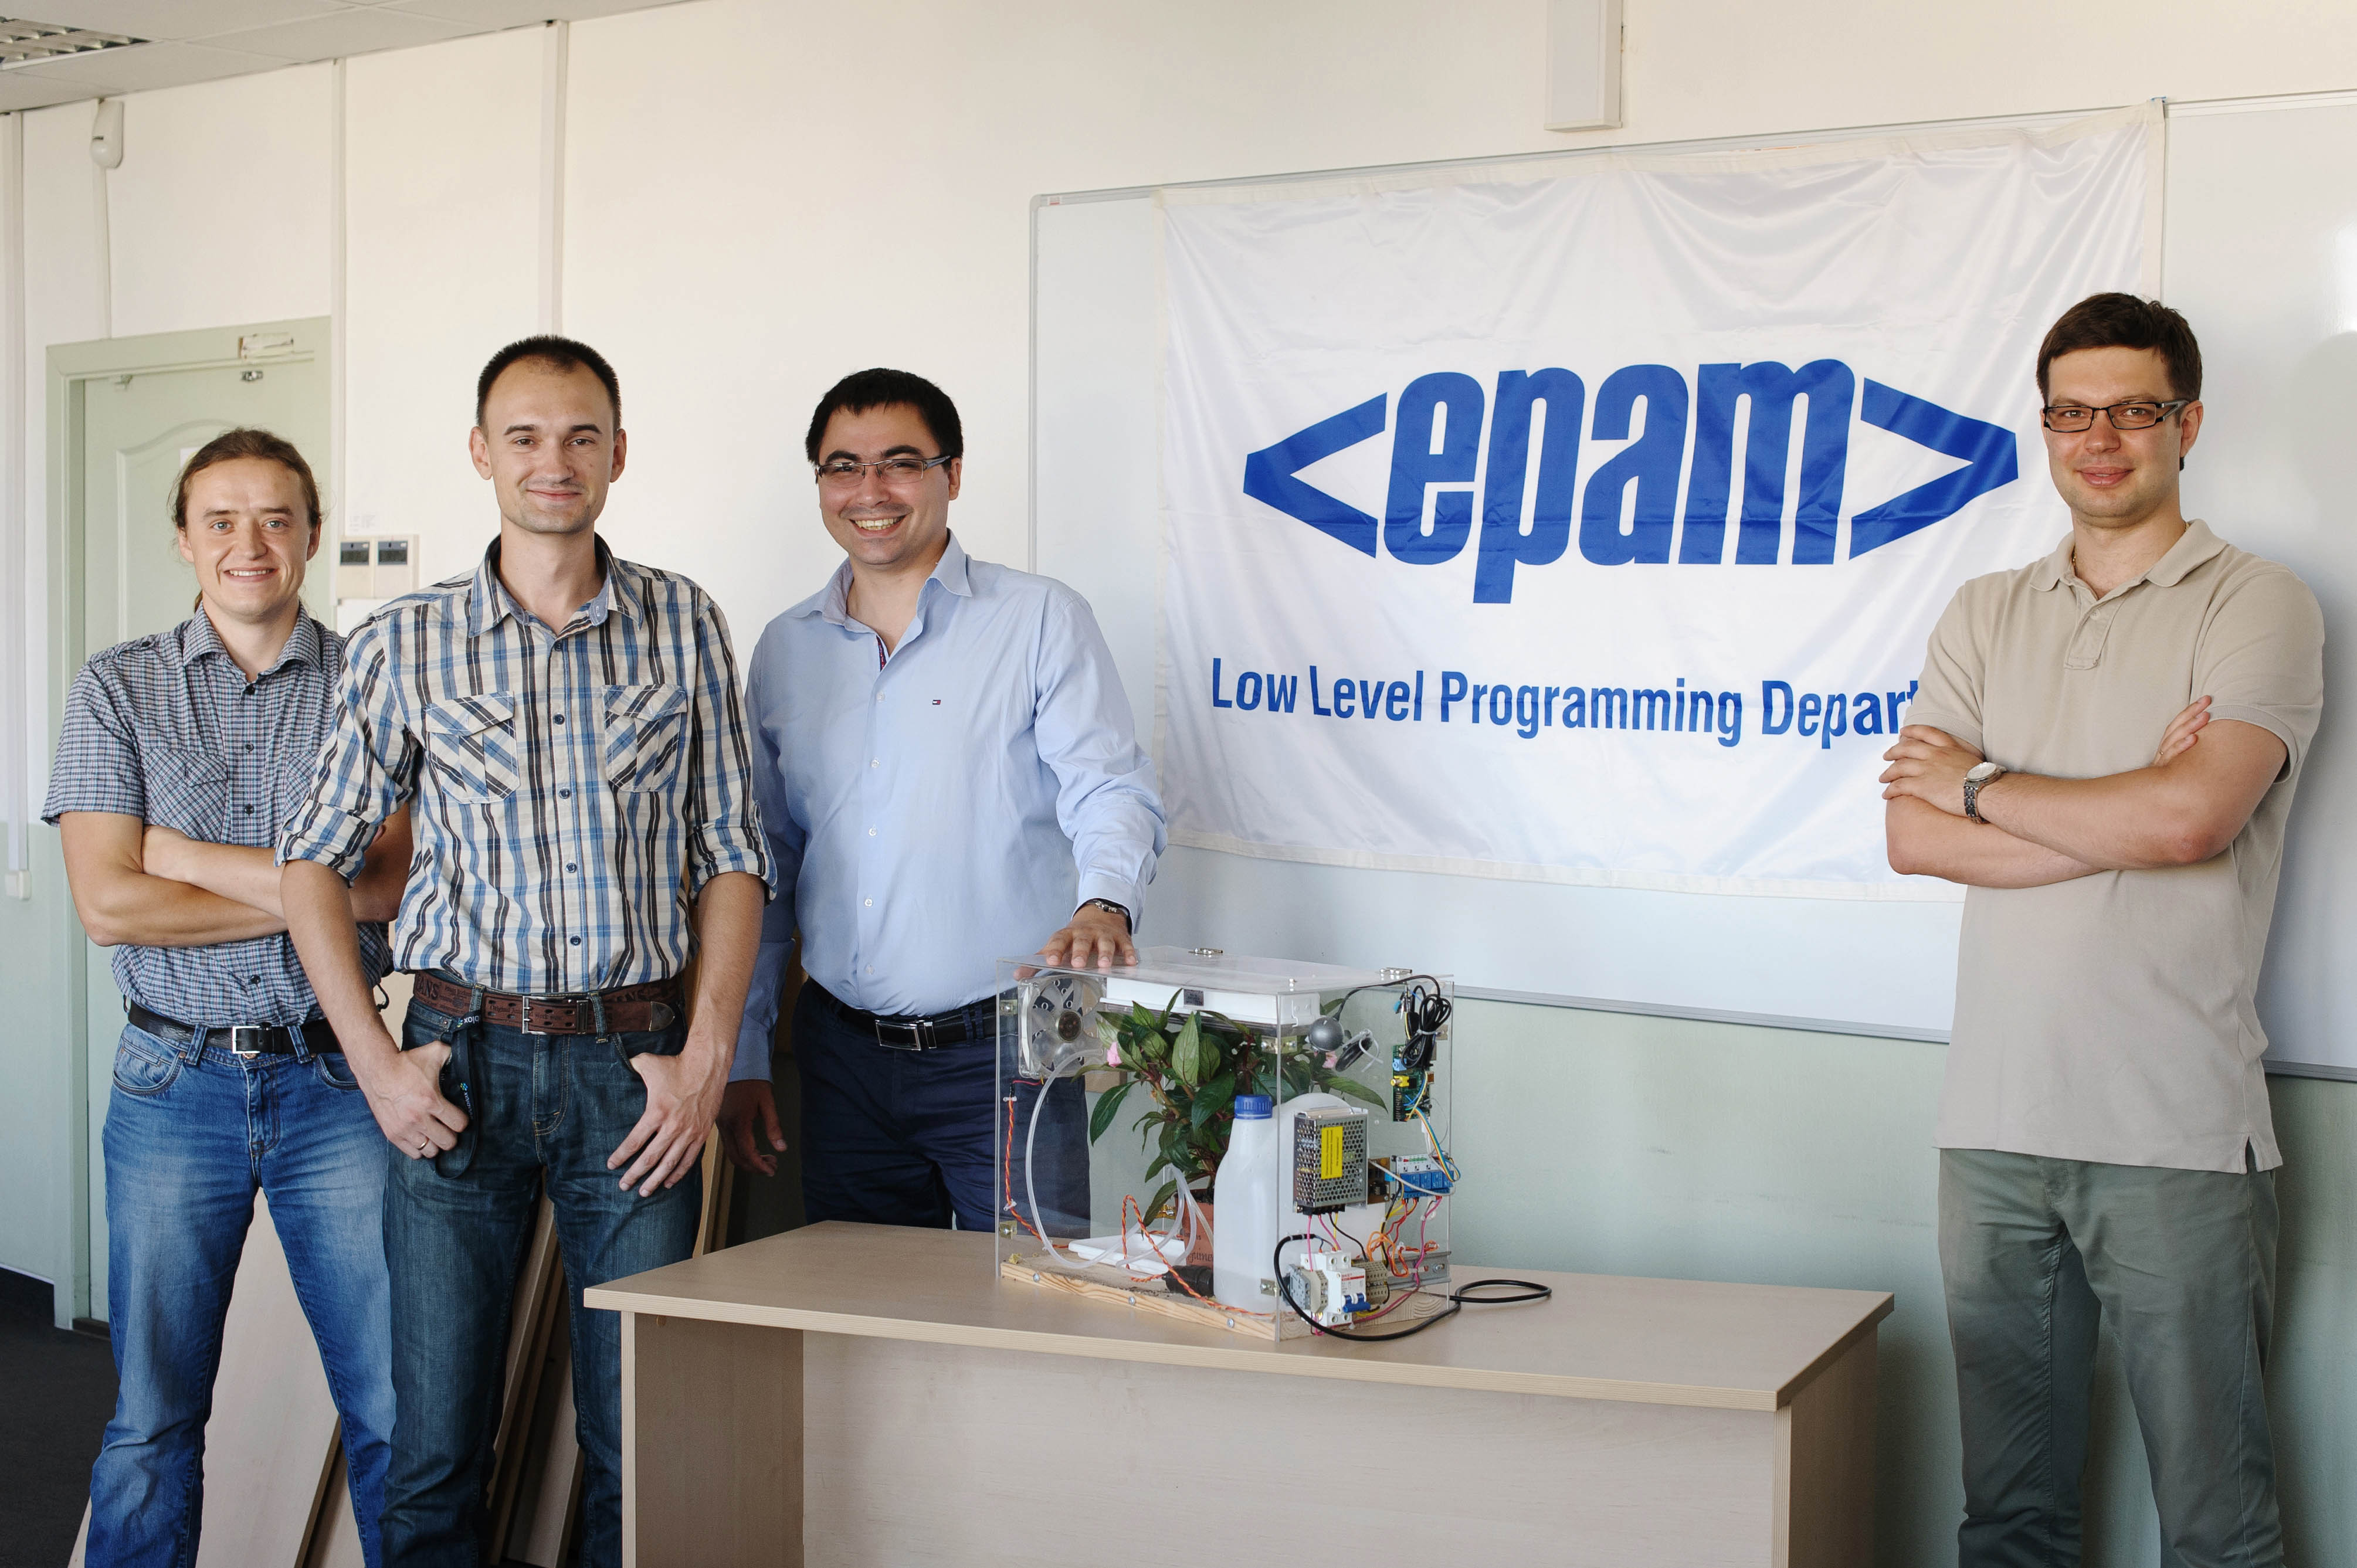
\includegraphics[scale=0.1]{Bilder/smartgreenhouse}
	\caption{Das Smart Greenhouse Entwicklerteam\cite{i:smartgreenhouse}}
	\label{f:smartgreenhouse}
\end{figure}

Das Team begann damit, als Grundlage den Raspberry Pi festzulegen. Hiermit besaßen sie einen gut ausgestatteten Einplatinencomputer mit 700 \ac{MHz} und 512 Mb Arbeitsspeicher, der mit 35 US\$ sehr preisgünstig ist. Doch bereits hiermit entstanden die ersten Bedenken. Um die Elektronik vor dem im Gewächshaus angebrachten Wässerungssystem zu schützen, musste alles gründlich isoliert und vor eindringendem Wasser geschützt werden.\\
Da die Pi4j Bibliothek nicht die nötigen Treiber bereitstellt, die zum Kommunizieren mit den im Gewächshaus angebrachten Feuchtigkeitssensoren benötigt sind, hat das Team eigene Treiber, sowie eine Linux-basierte Betriebssystemdistribution entwickelt, die speziell auf dieses Projekt ausgerichtet ist.\\
Um dies zu ermöglichen, holten sie sich die Hardwareexperten Vasili Slapik und Vladimir Redzhepov ins Team, die eine entscheidende Rolle in der Entwicklung des Projektes spielten.

Im fertiggestellten Projekt sind folgende Funktionen enthalten:\\

\begin{itemize} 
	\item Erstellung eines Belichtungsplans
	\item Erstellung eines Bewässerungsplans
	\item Temperaturkontrolle
	\item Luftfeuchtigkeitskontrolle
	\item Automatisches Management und ferngesteuerte Überwachung des aktuellen Gewächshauszustandes
	\item Automatische Erstellung eines Wachstumsverlaufs
	\item Schutz vor Überspannung / Stromausfall
\end{itemize}

Die Entwickler stellen dieses Projekt jedem Farmer kostenlos zur Verfügung. Da als Hardware nur ein Raspberry Pi, sowie weitere kostengünstige Komponenten benötigt werden, kann das Smart Greenhouse von Bastlern problemlos nachgebaut werden.
Das Betriebssystem, sowie die nötige Software kann aus der Dropbox des Entwicklerteams kostenlos heruntergeladen werden\cite{z:smartgreenhouse}.
